\documentclass[11pt]{article}
\usepackage[margin=1in]{geometry}
%\renewcommand{\baselinestretch}{1.8} 
%\usepackage{cite}
\usepackage[english]{babel}
\usepackage[sort, numbers, authoryear]{natbib}
\renewcommand{\arraystretch}{.5}
\usepackage{authblk}
\usepackage{setspace}
\usepackage{scalerel}
\usepackage{upgreek}
\usepackage{amssymb}
\usepackage{mathtools}
\usepackage{amsmath}
\usepackage{lscape}
\usepackage{tabls}
\usepackage{graphicx}
\usepackage{color}
\usepackage{url}
\usepackage{booktabs}
\usepackage{amsmath}
\usepackage{upgreek}
\usepackage{amssymb}
\usepackage{bm}
\usepackage{lscape}
\usepackage{pdfpages}
\usepackage{float}
\usepackage{fancyvrb}
\usepackage[hidelinks]{hyperref}






\newcommand\reallywidehat[1]{\arraycolsep=0pt\relax%
\begin{array}{c}
\stretchto{
  \scaleto{
    \scalerel*[\widthof{\ensuremath{#1}}]{\kern-.5pt\bigwedge\kern-.5pt}
    {\rule[-\textheight/2]{1ex}{\textheight}} %WIDTH-LIMITED BIG WEDGE
  }{\textheight} % 
}{0.5ex}\\           % THIS SQUEEZES THE WEDGE TO 0.5ex HEIGHT
#1\\                 % THIS STACKS THE WEDGE ATOP THE ARGUMENT
\rule{-1ex}{0ex}
\end{array}
}


\doublespacing

\usepackage{graphicx} % Required for inserting images

\title{SEI Redesign}
\author{Kim Larson}
\date{October 2025}

\begin{document}

\maketitle

\begin{abstract}
This is where we write the summary of what we found. \cite{kennedy2018evaluation}


\end{abstract}



\section{Introduction}


\begin{itemize}
    \item Why SEI's matter + long-standing critiques (validity/bias)
    
    \item Your contribution: a framework and prototype for an LLM-driven, dynamic student evaluation, an empirical study static vs. dynamic instrument.
\end{itemize}



Accreditation is 

\section{Background and Literature Review}


Institutions collect static student feedback \cite{ALHIJA200937}

Students provide longer comment feedback using computers than they did using pencil and paper \cite{}

Institutions also use focus groups\cite{Smithson01012000}

Students have bias \cite{stoesz2022bias}

Where does bias show up in traditional student evaluations of institution (SEI)? 
- Gender
- Discipline 
- Incentives to complete the form -- self serving (does it feel good to take it and reward the good / pushing the bad) or is it altruistic (will it help or punish the instructor, will it help or harm future classes) \cite{Hamilton01072002}





\section{Experiment Design and Proposal}
The current method - static with questions as current 

The proposed method - integrate the LLM into a survey for a class compared to prior years or within the same class 


\section{Results}

\section{Limitations}
Classes are small for graduate level classes compared to large institutions with large lecture halls. 

Student incentives to complete the survey - when surveys are anonymous, the 

\section{Conclusion}
This is a thing worth exploring to get more actionable insights from students. 

\bibliography{bibHere}{}

\bibliographystyle{apalike}

\end{document}


% Overflow
% \begin{figure}[H]
% \centering
% % 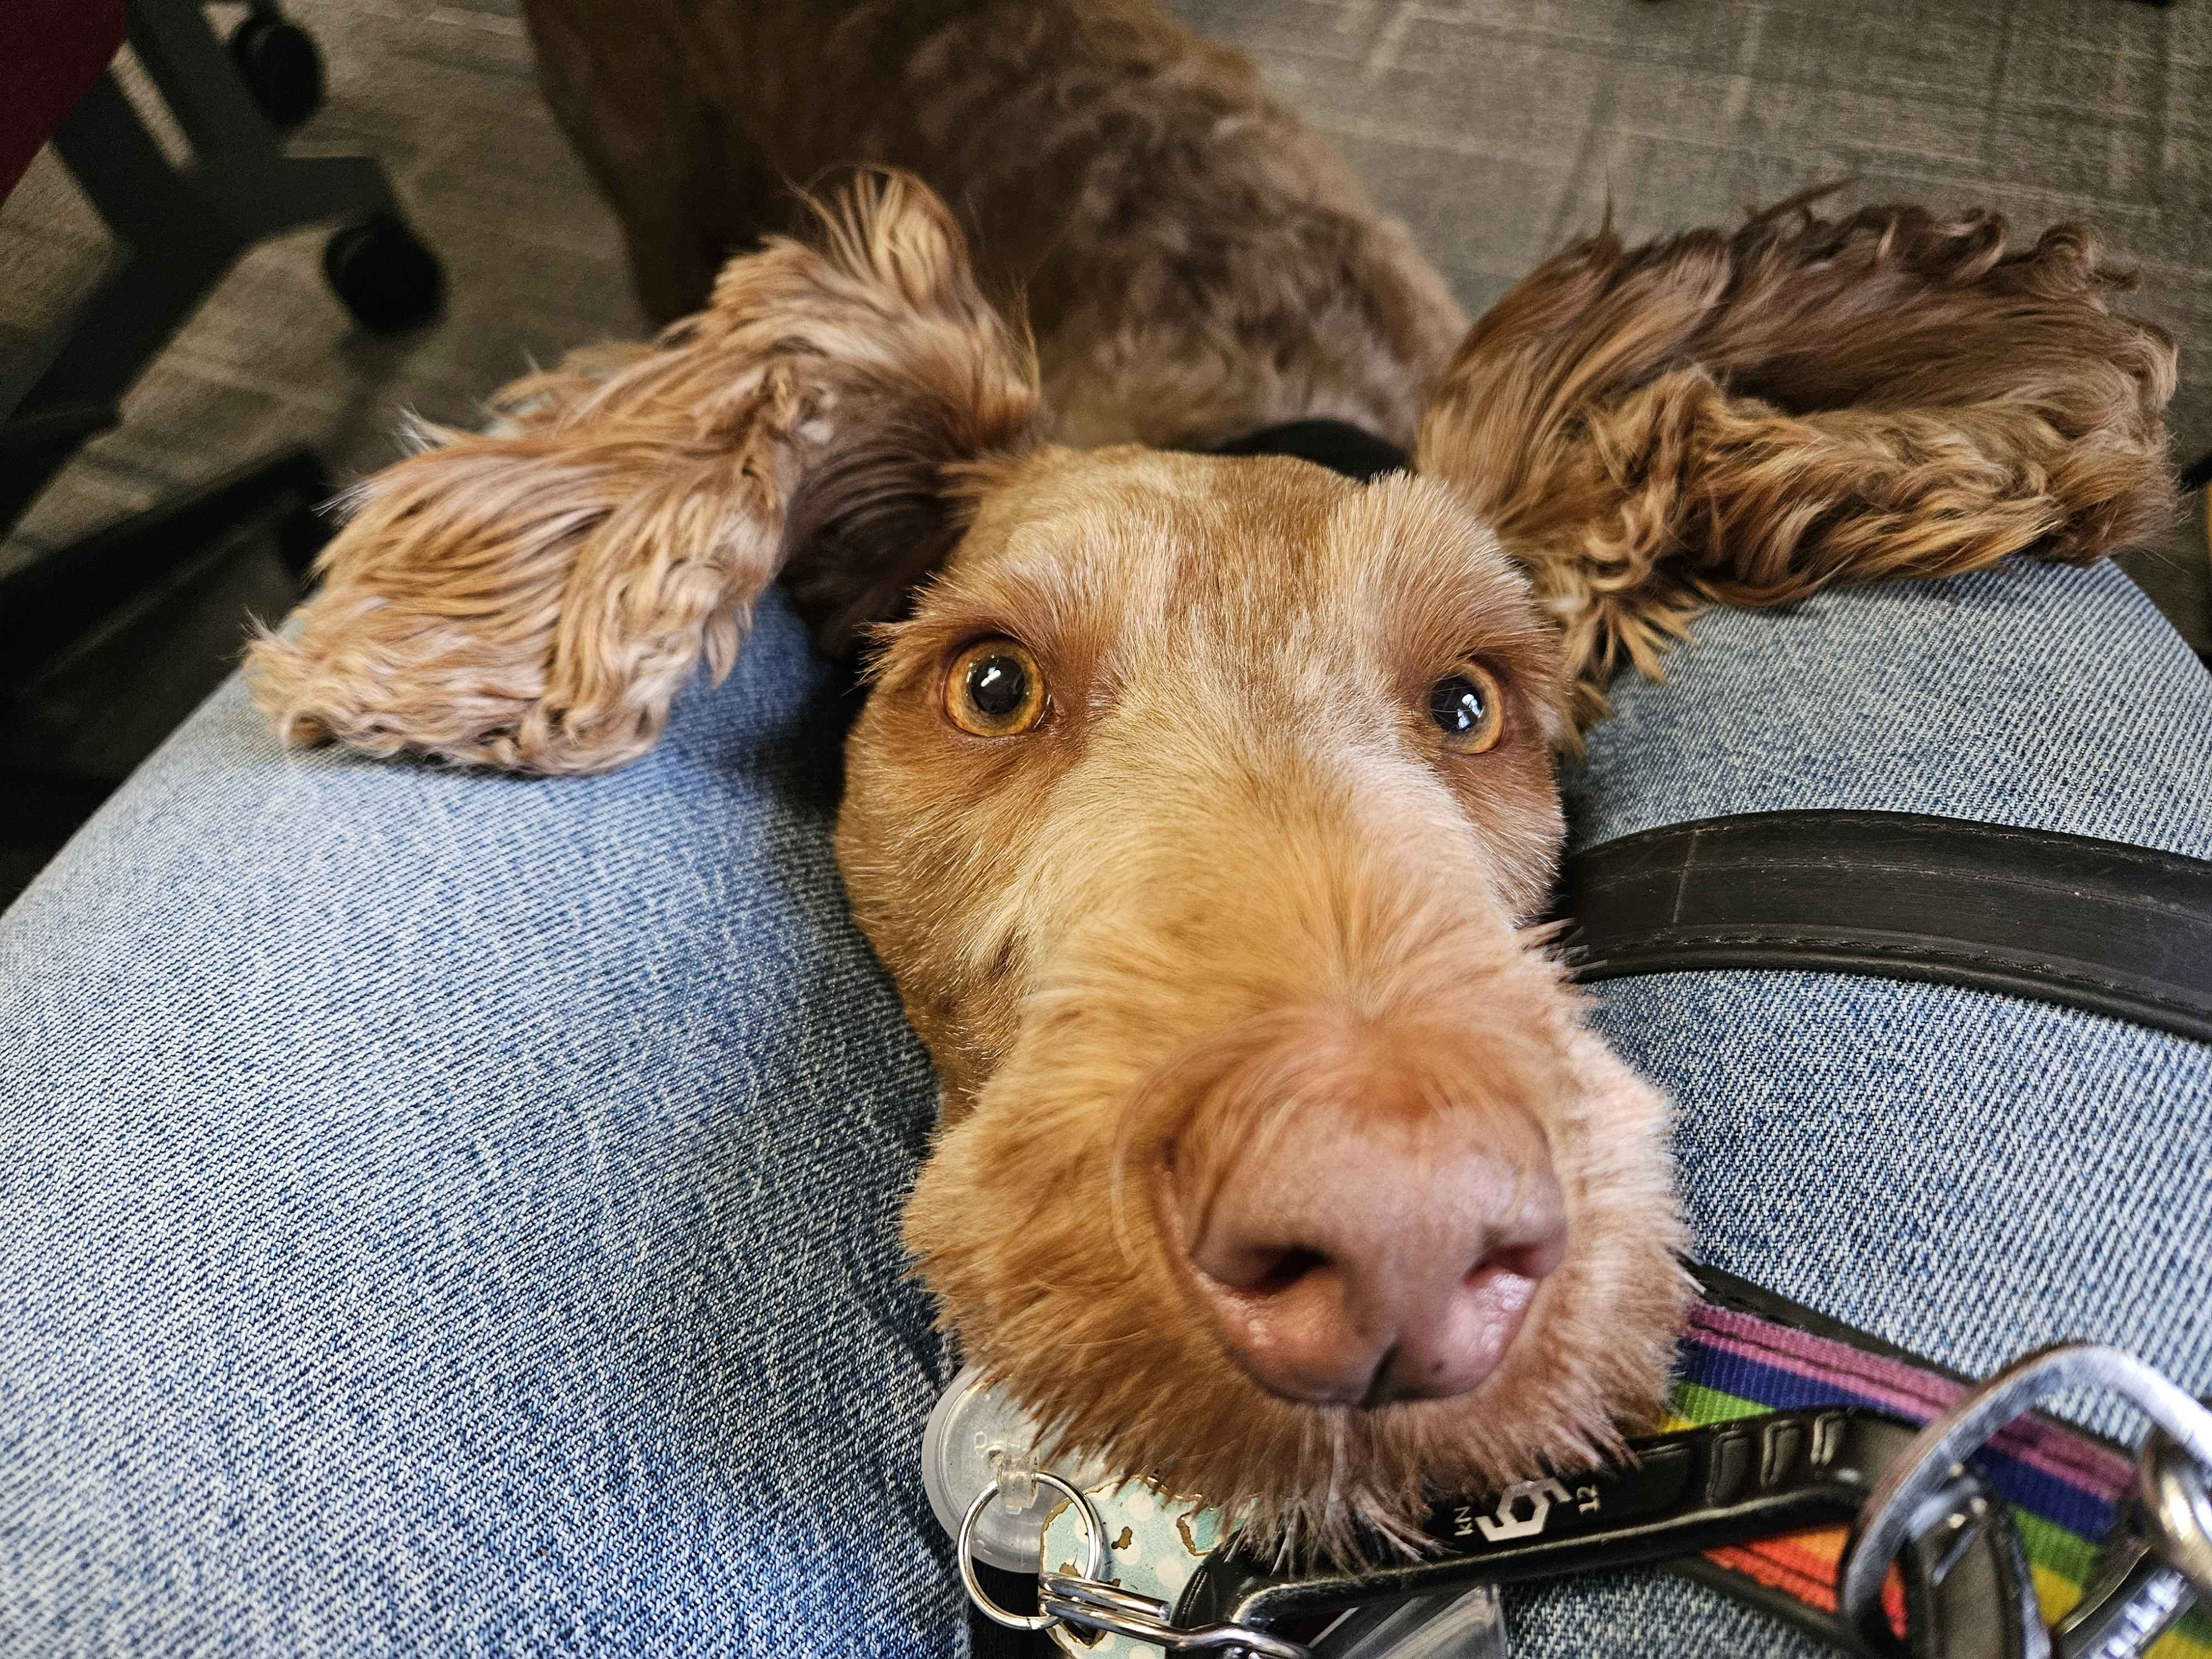
\includegraphics[width=0.5\linewidth]{Emmy.jpg}
% % \caption{That's a dog doing data science}
% \label{fig:gpig}
% \end{figure}